\documentclass[
% opciók nélkül: egyoldalas nyomtatás, elektronikus verzió
% twoside,     % kétoldalas nyomtatás
% tocnopagenum,% oldalszámozás a tartalomjegyzék után kezdődik
]{thesis-ekf}
\usepackage[T1]{fontenc}
\PassOptionsToPackage{defaults=hu-min}{magyar.ldf}
\usepackage[magyar]{babel}
\usepackage{mathtools, amssymb, amsthm, pdfpages}
\usepackage{enumitem, graphicx, listings, xurl, xcolor}
\lstset{
	language=Python,
%	literate={ö}{{\"o}}1{ü}{{\"u}}1{ó}{{\'o}}1{ő}{{\H o}}1{ú}{{\'u}}1{ű}{{\H u}}1{é}{{\'e}}1{á}{{\'a}}1{í}{{\'i}}1{Ö}{{\"O}}1{Ü}{{\"U}}1{Ó}{{\'O}}1{Ő}{{\H O}}1{Ú}{{\'U}}1{Ű}{{\H U}}1{É}{{\'E}}1{Á}{{\'A}}1{Í}{{\'I}}1
	xleftmargin=0.5cm,
	xrightmargin=0.5cm,
	breaklines,
	tabsize=4,
	showstringspaces=false,
	frame=tlbr,
	postbreak=\hbox{$ \color{red}\hookrightarrow\ $},
	backgroundcolor=\color{gray!30},
	rulecolor=\color{green!50!black},
	keywordstyle=\color{blue},
	commentstyle=\color{green!60!black},
	morekeywords={None},
	morekeywords=[3]{nx,append,items,values,previous},
	keywordstyle=[3]\color{cyan}
}
\footnotestyle{rule=fourth}

\newtheorem{tetel}{Tétel}[chapter]
\theoremstyle{definition}
\newtheorem{definicio}[tetel]{Definíció}
\theoremstyle{remark}
\newtheorem{megjegyzes}[tetel]{Megjegyzés}

\begin{document}
	\institute{Matematikai és Informatikai Intézet}
	\title{A kommunikációs gráfok modelljeinek vizsgálata Python programozási nyelvvel}
	\author{Mohai Ferenc\\programtervező informatikus BSc}
	\supervisor{Dr.~Kusper Gábor\\egyetemi docens}
	\city{Eger}
	\date{2022}
	
	\maketitle
	\tableofcontents
	
\chapter*{Bevezetés}
	\addcontentsline{toc}{chapter}{Bevezetés}
	Már a szakdolgozati szemináriumon, amikor hallottam Dr.~Kusper Gábor tanár úr magyarázatát a kutatásáról, annak eredményeiről, céljáról, felhasználásáról, nagyon megtetszett a téma.
	A \textsc{SAT} megoldó széles körű felhasználásáról beszélgettünk.
	Korábbi előadásokon, gyakorlatokon is voltak tanáraim, akik ezt a témát felvetették, és már akkoriban is felkeltette az érdeklődésemet.
	Amikor a szakdolgozatomhoz témát kellett választanom, nem volt kérdés, hogy számomra mi az érdekes téma, mi az amivel szívesen foglalkozom, és ami lehetőséget ad a fejlődésre is.

	Szaktársammal, Rajna Franciskával csak mi ketten érdeklődtünk ez iránt a téma iránt, így mindenki örömmel beszélte át a részleteket és közös megegyezéssel találtuk ki, hogy ki melyik ágát dolgozza fel a témának.
	Pozitív és energikus első benyomás után örömmel kezdtünk a munkának. Biró Csaba és Balla Tamás tanár urakkal dolgoztunk a témával kapcsolatos házi TDK-hoz hasonló előadásokon és kutatásokon \cite{am} vettünk részt. Az egyik alkalommal egy plakátot is készítettünk, ezekkel megalapozva egy lendületes kezdést.
	
	Megbeszéltük hol szorul fejlesztésre a \textsc{SAT} megoldó, melyik az a része, amin programozással tudok javítani. Tanáraim korábbi angol nyelvű publikációiból, azok általam magyarra fordított részeiből sikerült eljutni a megoldandó feladat megközelítéséhez. Ezek adtak eszközt a kezembe szakdolgozatom elkészítéséhez.
		
\chapter{Az alapok}
	
A munkámat tehát azzal kezdtem, hogy szakirodalmakat olvastam, fordítottam és értelmeztem, amiket korábban témavezetőim írtak, ez \az{\pageref{ssec-fogalmak}}.~és a \az{\pageref{sec-szakirodalom-forditas}}.~oldalon olvasható.
Anyagot gyűjtöttem és dolgoztam fel a \textsc{SAT} megoldókról.
Ezekben megjelentek különböző definíciók, mint \ref{def-tautologia}.~definíció a tautológia, \az{\ref{def-cnf}}.~definíció a \textsc{CNF}, és \az{\ref{def-dnf}}.~definíció a \textsc{DNF}, valamint programozási nyelv, mint a Python \az{\ref{kif-python-programnyelv}}.~szakaszban és a WolframAlpha válasz motor \az{\ref{kif-wolframalpha-hasznalata}}.~szakaszban. Az alábbiakban ezeket részletezem a szakdolgozatom megértéséhez.
	
\section{Fogalmak, definíciók a kommunikációs gráf felépítésének elemei}\label{sec-alap-fogalmak}

\begin{definicio}
	Atomi formula, röviden atom: Azt mondjuk, hogy egy szimbólum atomi formula, vagy atom, akkor és csak akkor, ha egy nem összetett kijelentést jelöl. Például a F szimbolum jelölheti ezt a kijelentést: Fúj a szél. Egy atom, pl. a fenti F atom, lehet igaz vagy hamis a két értékű 0.-ad rendű matematikai logikában. Az igaz értéket általában az \emph{I} szimbolum jelöli, míg a hamis értéke a \emph{H}, de szoktuk használni az angol megfelelőjét is a \emph{T} és \emph{F} betűket, amelyek a ,,true'' és a ,,false'' szavak kezdőbetűjéből jönnek.
\end{definicio}

\begin{definicio}		
	Jól formázott formula, röviden formula: Azt mondjuk, hogy egy szimbólumsorozat jól formázott formula, vagy formula, akkor és csak akkor, ha a szimbólumsorozat a következő alakok egyikében van:
	\begin{enumerate}[label=\textit{(\alph*)}]
		\item A, ahol A egy atom;
		\item $ \neg A $, ahol A egy formula;
		\item $ (A \wedge B) $, ahol A és B formulák;
		\item $ (A \vee B) $, ahol A és B formulák;
		\item $ (A \implies B) $, ahol A és B formulák;
		\item $ (A \Leftrightarrow B) $, ahol A és B formulák.
	\end{enumerate}
	Minden formula a fenti esetek véges sokszori alkalmazásával áll elő.
\end{definicio}

\begin{megjegyzes}
	Logikai operátor: A logika nyelvének része a logikai összekötő jelek, vagy más néven logikai operátorok. Mi a következő logikai operátorokat használjuk:
	\begin{enumerate}
		\item Negáció, jele: $ \neg $
		\item Implikáció, jele: $ \implies $
		\item Ekvivalencia, jele: $ \equiv $
		\item Konjunkció, jele: $ \wedge $
		\item Diszjunkció, jele: $ \vee $
	\end{enumerate}
\end{megjegyzes}

\begin{definicio}
	Literál: Azt mondjuk, hogy egy formula literál, akkor és csak akkor, ha atom, vagy atom negáltja.
	Egy \emph{literál} pozitív, ha atom, illetve negatív, ha atom negáltja. 
\end{definicio}

Példa a literálokra: $ a,\neg a,b,\neg b,\dots $, ahol $a$ egy pozitív literál, $\neg a$ egy negatív literal, stb.

\begin{definicio}
	Interpretáció: Azt mondjuk, hogy egy J hozzárendelés egy F formula egy interpretációja, akkor és csak akkor, ha a J az F minden atomjához vagy az igaz, vagy a hamis értéket rendeli, de ezek közül csak az egyiket.
\end{definicio}

\begin{definicio}
	Klóz, angolul clause: A klóz literálok halmaza, amelyet úgy interpretálunk, hogy a halmazban lévő literálok diszjunkciója. Például:
	\begin{enumerate}
		\item $ \{a,\neg b\} $, ami ezt a formulát jelöli: $a \vee \neg b$
		\item $ \{a,b,c\} $
		\item $ \{a\} $
	\end{enumerate}
\end{definicio}

\begin{megjegyzes}
	Habár a definíció megengedi, hogy egy klózon belül valamely atom
	megjelenjen negatív és pozitív literálként is, például: $ {a,\neg a}$, 
	viszont az ilyen klózokat nem használjuk, mert ezek mindig igazak.
\end{megjegyzes}

\begin{definicio}\label{def-cnf}
	Konjunktív normál forma, röviden \textsc{KNF}, angolul conjunctive normal form, röviden \textsc{CNF}: Azt mondjuk, hogy egy logikai formula konjuktív normál formában van, akkor és csak akkor, ha egy vagy több klózból áll, amelyeket
	konjunkcióval kötünk össze.
\end{definicio}

Példa egy kojunktív normál formában lévő formulára: $ (A \vee B \vee C \vee X) \wedge (\neg A \vee \neg B \vee \neg C \vee X) \wedge (\neg A \vee B \vee \neg X) $. Ez egy KNF formula, mivel zárójelen belül diszjunkció köti össze a literálokat, a klózok között pedig konjunkció található.

\begin{definicio}\label{def-dnf}
	Diszjunktív normál forma, angolul disjunctive normal form, röviden \textsc{DNF}: Azt mondjuk, hogy logikai formula diszjunktív normál forma, akkor és csak akkor, ha literálok konjunkciójának diszjunkciója.
\end{definicio}


	Példa egy DNF formulára: $ (A \wedge B \wedge C \wedge X) \vee (\neg A \wedge \neg B \wedge \neg C \wedge X) \vee (\neg A \wedge B \wedge \neg X) $. Ez egy DNF formula, mivel zárójelen belül konjunkció köti össze a literálokat, a klózok között pedig diszjunkció található.


\begin{definicio}\label{def-tautologia}
	Logikai törvény, más néven tautológia: Azt mondjuk, hogy az F formula logikai törvény, vagy tautológia, akkor és csak akkor, ha F minden interpretációjában igaz.
\end{definicio}

\begin{definicio}
	Logikai ellentmondás, angolul contradiction, unsatisfiable formula, röviden UNSAT: Azt mondjuk, hogy az F formula logikai ellentmondás, akkor és csak akkor, ha F minden interpretációjában hamis.
\end{definicio}

\begin{definicio}
	Kielégíthető, angolul satisfiable formula, röviden \textsc{SAT}: Azt mondjuk, hogy az F formula kielégíthető, akkor és csak akkor, ha F legalább egy interpretációjában igaz.
\end{definicio}

\begin{definicio}
	Hamissá tehető, angolul falseable formula: Azt mondjuk, hogy az F formula hamissá tehető, akkor és csak akkor, ha F legalább egy interpretációjában hamis. 
\end{definicio}

\begin{megjegyzes}
	Kielégítő ellentéte a logikai ellentmondás, mivel ha valami nem kielégíthető, akkor abból következik, hogy minden interpretációjában hamis, azaz logikai ellentmondás.
	Hamissá tehető ellentéte a logikai törvény, mivel ha valami nem hamissá tehető, akkor abból következik, hogy minden interpretációjában igaz, azaz logikai törvény.
\end{megjegyzes}

Igazság tábla: Oszloponként tartalmazza az összes atomot, ami a formulánkban van, és az utolsó oszlopban magát a formulát is. Soronként minden atomhoz értéket rendel, minden lehetséges kombinációban, és a formulába behelyettesítve kiszámítja a formula értékét. Az eredményét az utolsó oszlopból olvashatjuk ki.

Logikai törvény, tautológia: Ezek segítségével felírhatunk olyan formulákat, és igazság táblákat, amelyek minden lehetséges esetre igaz értéket adnak eredményül. Az eredményekből könnyebben átláthatjuk, ha tautológiát kapunk.

\label{pelda-tautologia}
	Példa tautológiára és igazság táblára: 
		
	Legyen $ a $ egy atom, akkor a következő formula eredménye mindig igaz lesz: $ a\vee\neg a $
	
	\begin{tabular}{|c|c|}
		\hline
		$ a $ & $ a\vee\neg a $ \\
		\hline
		I & I \\
		\hline
		H & I \\
		\hline
	\end{tabular}

	Legyen $ x $ és $ y $ egy-egy atom, akkor a következő formula eredménye mindig igaz lesz: $ x \Leftrightarrow y\vee \neg(x\Leftrightarrow y) $
	
	\begin{tabular}{|c|c|c|}
		\hline
		$ x $ & $ y $ & $ x\Leftrightarrow y\vee\neg(x\Leftrightarrow y) $ \\
		\hline
		I & H & I \\
		\hline
		H & I & I \\
		\hline
	\end{tabular}

\textsc{SAT} probléma: A logikai kielégíthetőség egy olyan probléma, ami azt határozza meg, hogy létezik olyan interpretációja egy logikai formulának, ami kielégíti az adott logikai formulát.

\textsc{SAT} megoldó, angolul \textsc{SAT} solver: \textsc{SAT} problémák megoldására képes. Eredményül egy igaz vagy hamis értéket ad, ami annyit jelent, hogy a kapott probléma kielégíthatő-e vagy sem. Ha kielégíthető, megadj egy interpretációt is, amiben a formula igaz.

\subsection{Tanáraim útmutatása a szakirodalom terén} \label{ssec-graf-alapok}
\begin{definicio}
	Azt a konstrukciót, hogy $\mathcal{D}=(\mathcal{V},\mathcal{E})$, irányított gráfnak nevezzük, ahol $ \mathcal{V} $ a csúcsok halmazát jelöli, $\mathcal{E}$ pedig az élek halmazát. Egy él csomópontok rendezett párja, az $(a,b)$ irányított élt úgy jelöljük az irányított gráfban, hogy $a \rightarrow b$, és azt is mondhatjuk hogy az $a$ gyermeke a $b$ csomópont. Ha $(a,b)$ eleme az $\mathcal{E}$ halmaznak, akkor azt mondjuk, hogy $(a,b)$ egy éle a $\mathcal{D}$ irányított gráfnak.
\end{definicio}
\begin{definicio}
	Egy irányított gráf teljes, akkor és csak akkor, ha minden pár külön álló csúcsokból össze van kötve egy pár egyedi éllel (eggyel minden irányba). Egy irányított gráf erősen összetett, vagy erősen irányított gráf, akkor és csak akkor, ha van út minden csúcsból minden más csúcsba. Vegyük észre, hogy a teljes gráf egyben erős is; továbbá, az erősen irányított gráf tartalmaz egy kört, ami tartalmaz minden csúcsot \cite{am}.
\end{definicio}

\begin{definicio}
	Erősen összetett gráf, más néven erős gráf: Azt mondjuk, hogy egy gráf erős gráf, akkor és csak akkor, ha van út minden csúcs pár között.
\end{definicio}
	
	\begin{definicio}
		Erősen összetett komponens, más néven erős komponens, angolul strongly connected component, röveiden \textsc{SCC}: Azt mondjuk, hogy egy részgráf erősen összetett komponens, akkor és csak akkor, ha egy irányított gráfnak a legnagyobb, erősen összekötött részgráfja.
	\end{definicio}
	
	\begin{definicio}
		Fekete hozzárendelés, más néven fekete klóz: Azt mondjuk, hogy egy klóz fekete klóz, akkor és csak akkor, ha a gráf minden csúcsának a negáltja megtalálható benne.
	\end{definicio}
	
	\begin{definicio}
		Fehér hozzárendelés, más néven fehér klóz: Azt mondjuk, hogy egy klóz fehér klóz, akkor és csak akkor, ha a gráf minden csúcsa megtalálható benne.
	\end{definicio}

 	\section{Gráf alakzatok létrehozása}

	A drawio nevű weboldalon \cite{link-drawio} elérhető egy \textsc{XML} alapú képszerkesztő. Ez egy olyan webes grafikus felületet ad, ami gráfok, diagramok, uml-ek, use-case ábrák, képek és még sok más forma megszerkesztését teszi lehetővé. Ha akarjuk, le is tölthetjük ingyenesen az asztali alkalmazást, ami szélesebb körben, gyorsabban és precízebben működik, mint a webes felület. Gyorsabb a fájlok kezelése, szerkesztése is.
	
	Rengeteg alapértelmezett alakzatot találunk benne, használata egyszerű, és könnyen elsajátíthatja a felhasználó. Körülbelül 3 éve hallottam erről az alkalmazásról, talán Troll Ede tanár úr mutatta be nekünk még a ,,Bevezetés az informatikába'' órán. Azóta rengeteg uml-t, use-case-t és egyéb hasznos dolgot szerkesztettem már meg, csakúgy, mint a jelenlegi dokumentumban található összes gráfot.
	
	\section{Logikai formulák ellenőrzése}
	
	A logikai formulák ellenőrzéséhez a WolframAlpha válasz motort választottam, melynek nyelve a Wolfram, ami egy általános, több paradigmás programozási nyelv. Ez a nyelv a hangsúlyt a szimbolikus számításra, a funkcionális programozásra, a szabályalapú programozásra helyezi, valamint képes tetszőleges struktúrákat és adatokat alkalmazni. Ezekre az alapokra épül a WolframAlpha tudásszámító és válasz motor. Képes közvetlenül válaszolni a tényszerű kérdésekre azáltal, hogy külső forrásból származó adatokból számítja ki a választ.
	
	Mi arra tudjuk használni, a saját weboldalán keresztül \cite{link-wolframalpha}, hogy a beviteli mezőben logikai formulát adunk át neki. Válasznak visszaadja megformázva, amit bevitelként adtunk, valamint annak igazság tábláját, normál formáit, logikai áramkörét, Venn diagramját és az igazságsűrűségét.
	
	Így könnyen leellenőrizhető, hogy a logikai formula, amit beírtunk az tautológia-e. Ezt az igazságtábla utolsó oszlopából állapíthatjuk meg.
	
		\subsection{A WolframAlpha válaszmotor használata} \label{kif-wolframalpha-hasznalata}
	Alapértelmezésben akár szavak keresésére is alkalmas, nagyon széleskörű, intelligens keresőmotor. Képes megkeresni, akár egy szónak a rímpárját is. Ugyanakkor képes az egészen egyszerű és a bonyolult matematikai képleteken át, a nagyon összetett logikai formulákig bármire válaszolni. Ehhez csak meg kell tudni adni, vagy kiválasztani a megfelelő formátumot, amiben dolgozva a keresés a számunkra kívánt eredményt adja. Egy szó begépelésével, annak jelentését adja vissza, a hozzá tartozó szinonimákat, nyelvtani felépítését, az évek alatt változó használatát, és még sok minden mást. Ha matematikai, műveleti jelekkel teletűzdelt értelmezhető képletet írunk be, akkor azt adott értékkel kiszámolja, és a hozzá köthető részeredményeket, lebontást, grafikonokat is megadja a válaszban.
	
	A mi esetünkben a logikai képletek megformázása a legérdekesebb használati eset. Az alapműveletek jeleit átírja a saját nyelvén megformázott bemenetre, és ezt szövegesen is leírja. Ebben a felsorolásban a műveleti jeleket szó szerint kell beírni az idézőjelek közé:
	\begin{itemize}
		\item negálás $ = $ ,,not A'' példa: $ \neg A $, \textsc{Not A}
		\item ,,vagy'' művelet $ = $ ,,A or B'' példa: $ A\vee B $, \textsc{A Or B}
		\item ,,és'' művelet $ = $ ,,A and B'' példa: $ A\wedge B $, \textsc{A And B}
		\item implikáció $ = $ ,,A => B'' példa: $ A\Rightarrow B $, \textsc{A Implies B}
		\item ekvivalencia $ = $ ,,A <=> B'' példa: $ A\Leftrightarrow B $, \textsc{A Equivalent B}
	\end{itemize}
	Természetesen zárójelekkel kombinálva már használhatjuk is bonyolultabbnál bonyolultabb képletek kiszámítására.
	
	Kiszámítja, hogy a beadott érték, formula, képlet tautológia-e. Láthatjuk a \textsc{CNF, DNF, ANF, NOR, NAND, AND, OR} minimális- és esetleg egyéb \textsc{ESOP, implikáció, ITE, BDT} formákra alakítva milyen eredményt ad. Készít róla logikai áramkört, Venn diagramot, és igazságsűrűség kimutatást is.
	
	Ezeket természetesen ingyenesen kapjuk, ha előfizetünk, akkor jobb minőségű, kinagyítható, szerkeszthető képleteket kapunk, nemcsak egy rögzített méretű képben megadott eredményt. Hosszabb eredmények esetén előfordul, hogy a minimális formákat sem adja eredményül, természetesen prémium felhasználóként ezeket akár kijelölhető szövegként is megkapjuk.
	
	\section{A Python programozási nyelvről}\label{kif-python-programnyelv}
	A Python egy magas szintű programozási nyelv, ami a funkcionális, az objektumorientált, az imperatív és a procedurális programozási paradigmákat támogatja. Azaz egy olyan több paradigmás nyelv, ami függvényeket, eljárásokat, metódusokat, változókat, használ, ezekkel változtatja meg a program állapotát. Bár dinamikusan típusos nyelv, mégis hibát dob a nem jól definiált műveletek használatára. Például nem lehet hozzáadni számot szöveghez, viszont dinamikus, mert a változóknak csak nevük van, és ha véletlenül ugyanazzal a névvel egy másik típust akarunk használni, azt felülírja, és az utoljára értékül kapott típust használja. Fontos a szintaxisra nézve, hogy minden behúzás jelentős, mivel ezeket használja a kódrészek csoportosítására. Hivatkozás számolást (angolul reference counting) és körészlelő szemétgyűjtést (angolul garbage collection GC) alkalmaz a memória visszaigényléséhez. Széleskörű az alapkönyvtár készlete, azaz sok importálható osztály van, amit más már megírt előttünk. Ez annak köszönhető, hogy modulokon keresztül nyújthatóvá tették az egész nyelvet. Dinamikus névmeghatározást használ, ami a késői kötésnek, vagy lusta kiértékelésnek köszönhetően a program futása közben köti össze a neveket és a metódusokat. Funkcionális függvényei is vannak, mint a \texttt{filter}, \texttt{map} és \texttt{reduce}, implementálva vannak fejlett listák (angolul list comprehension), szótárak, halmazok, generátor, valamint iterátor kifejezések is. Két alapkönyvtára van a \texttt{functools} és az \texttt{itertools}. Utóbbit én is használom a programomban, de ezen kívül még a gráfokhoz kidolgozott \texttt{NetworkX} és \texttt{Pylab} könyvtárakat is használom.
	
	Amikor először megnyitjuk a programot, akkor egy nagyon leegyszerűsített felhasználói felülettel találkozunk. Egyszerű benne az importálás, csak behúzásokkal van rendezve, nagyon tiszta a kódolási környezet. A nyelv megírásakor az volt a cél, hogy minél kevesebb időt kelljen a programkörnyezet kitalálásával tölteni, és a felhasználók munkájukat könnyen, átláthatóan végezhessék, szinte csak a célra kell fókuszálni, ahhoz hogy az adott problémát a programozási nyelvvel megoldhassuk. Kitűnően érvényesül a Python alapelve, ami a minél letisztultabb program struktúra létrehozása. Rengeteg kiegészítő könyvtára van, ami a széleskörű felhasználást segíti elő, azonban igazából a fájlok kezelésére, rövid, tömör kód megírására a legalkalmasabb. Használatával arra ösztönöz, hogy egy programrészletet ne gondoljunk túl, törekedjünk tiszta kód írására.
	
\chapter{Kutatás}
	\section{A gyenge modell fogalma}\label{sec-szakirodalom-forditas}
	
	\Az{\ref{sec-alap-fogalmak}}.~fejezetben már kifejtettem a logika alapjait. Ebben a fejezetben \az{\cite[Kusper Gábor és társai]{am}}-nak cikkéből, valamint \az{\cite[Kusper Gábor diploma munkája]{sat-solving-50}} az, amiből konzulensem javaslatára szakirodalom részleteket fordítottam le magyar nyelvre.
	
	\label{ssec-fogalmak}
	%todo nézd át a hivatkozásokat, legyenek értelmesebbek. 
	% A fordításokat pláne nézd át!
	A klózok itt literáljaik diszjunkciójaként vannak értelmezve. A hozzárendelések pedig literáljaik konjunkciójaként.
	
	Ha egy klóz vagy egy hozzárendelés pontosan \emph{k} literált tartalmaz, akkor \emph{k-klóznak}, vagy \emph{k-hozzárendelésnek} nevezzük. Egy 1-klózt \emph{egységnek}, egy 2-klózt \emph{bináris klóznak} nevezünk. Egy \emph{k-}\textsc{SAT} \emph{probléma} egy olyan klózhalmaz, ahol a klózoknak legfeljebb \emph{k} literálja van. Egy klóz a klózhalmazból, akkor és csak akkor egy \emph{teljes-hosszú klóz}, ha tartalmaz minden változót a klózhalmazból.
	
	Definiáljunk néhány kiegészítő függvényt. Ha $ C $ egy klóz, akkor legyen $ V(C) $ azon változók halmaza, ami feltűnik $ C $-ben, legyen $ N(C) $ a negatív literálok halmaza $ C $-ből, és legyen $ P(C) $ a pozitív literálok halmaza $ C $-ből. Tudjuk hogy $ C=N(C)\cup P(C)$, $V(N(C))\cap V(P(C))=\emptyset $, és $ P(C)=V(P(C)) $.
	
	Két intuitív fogalmat használunk: \textsc{NNP} klózt, és \textsc{NPP} klózt. Egy klóz akkor és csak akkor \textsc{NNP} klóz, ha pontosan egy pozitív literált tartalmaz. Egy klóz akkor és csak akkor \textsc{NPP} klóz, ha pontosan egy negatív literált tartalmaz.
	
	Ha $ a $ egy literál az $ S $ klózhalmazban, és $ \neg a $ literál nincs benne $ S $-ben, akkor azt mondjuk, hogy $ a $ egy tiszta literál $ S $-ben.
	
	A negációja $ H $ halmaznak $ \neg H $-val van jelölve, ami azt jelenti, hogy $ H $ minden eleme negálva van. Vegyük figyelembe, hogy $ \neg\neg H=H $.

	Legyen $ V $ a változók halmaza egy klózhalmazból véve. Azt mondjuk, hogy $ WW $ a \emph{fehér klóz}, vagy a \emph{fehér hozzárendelés} a $ V $ változóira, akkor és csak akkor, ha $ WW=V $. Azt mondjuk, hogy $ BB $ a \emph{fekete klóz} vagy a \emph{fekete hozzárendelés}, $ V $ változóira, akkor és csak akkor, ha $ BB =\neg V$. Például ha $ V=\{a,b,c\} $, akkor $ WW=\{a,b,c\} $, és $ BB=\{\neg a,\neg b,\neg c\} $.
	
	Azt mondjuk, hogy $ C $ magába foglalja $ D $ klózt, akkor és csak akkor, ha $ C $ részhalmaza $ D $-nek.
	
	Azt mondjuk, hogy $ S $ klózhalmaz \emph{magába foglalja} $ C $-t, akkor és csak akkor, ha $ S $-ben van olyan klóz, ami magába foglalja $ C $-t. Logikai jelölése: $ S $ \emph{magába foglalja} $ C \Leftrightarrow\exists D(D\in S\wedge D\subseteq C) $.
	
	Azt mondjuk, hogy $ C $ klózzal \emph{jár} $ S $ klózhalmaz, akkor és csak akkor, ha minden teljes hosszú klóz, amit magába foglal $ C $ azt $ S $ is magába foglalja. A logikai értelmezése ennek a fogalomnak a következő: $ C $-vel jár $ S $, akkor és csak akkor, ha $ C $ egy logikai következménye $ S $-nek. A magába foglalt klózokat is beleértve.

	Azt mondjuk, hogy $ C $ klóz \emph{független} $ S $ klózhalmazban, akkor és csak akkor, ha $ C $-vel nem jár $ S\setminus\{C\} $. Egy teljes hosszú klóz független egy klózhalmazban, akkor és csak akkor, ha semmi nem foglalja magába.

	Azt mondjuk, hogy $ M $ hozzárendelés egy \emph{megoldás} $ S $ klózhalmazra nézve, akkor és csak akkor, ha minden $ C\in S $-re igaz, hogy $ M\cap C\ne \{\} $.

	Azt mondjuk, hogy $ S $ klózhalmaz egy \emph{Fekete-Fehér} \textsc{SAT} \emph{probléma}, akkor és csak akkor, ha csak két megoldása van a fehér $ (WW) $ és a fekete $ (BB) $ hozzárendelés.

	Azt mondjuk, hogy $ A $ és $ B $ klózhalmazok ekvivalensek, akkor és csak akkor, ha mindkettőnek ugyanaz a megoldás halmaza. Azt mondjuk, hogy $ A $ klózhalmazzal jár $ B $ klózhalmaz, akkor és csak akkor, ha $ A $-hoz tartozó megoldások halmaza tartalmazza a $ B $-hez tartozó megoldás halmazt, azaz $ A $-nak nem lehet más megoldása, csak $ B $. Ez a fogalom a következőképpen van jelölve: $ A\geq B $. Vegyük figyelembe, ha $ A $ magába foglalja $ B $ minden klózát, akkor $ A\geq B $.

	Azt mondjuk, hogy $ A $ erősebb $ B $-nél, akkor és csak akkor, ha $ A\geq B $ és $ A $ és $ B $ nem egyenlőek. Ez a fogalom a következőképpen van jelölve: $ A>B $.

	Az irányított gráfot a \pageref{ssec-fogalmak}.~oldalon a \ref{ssec-fogalmak}.~fejezetben már definiáltam.
	
	Azt mondjuk, hogy $ \mathcal{D} $ egy kommunikációs gráf, akkor és csak akkor, ha minden $ a $-ra $ \mathcal{V} $-ben igaz, hogy $ (a,a) $ nincs benne $ \mathcal{E} $-ben, és ha $ x $ eleme $ \mathcal{V} $-nek, akkor $ \neg x $ nem lehet $ \mathcal{V} $ eleme. Szükségünk van erre a megszorításra, mert $ \mathcal{D} $-ből egy logikai formulát generálunk. Ha kommunikációs gráfokról beszélünk, akkor gyakran használjuk a csomópont kifejezést, a csúcs szinonimájaként.

	Egy út $ a_1 $-től $ a_j $-ig a $ \mathcal{D} $ irányított gráfban olyan csúcsok sorrendje $ a_1,a_2,\dots,a_j $, ami minden egyes $ i\{1,\dots,j-1\} $-re igaz, hogy $ (a_i,a_(i+1)) $ egy éle $ \mathcal{D} $-nek. Egy út $ a_1 $-től $ a_j $-ig $ \mathcal{D} $ irányított gráfban egy kör, akkor és csak akkor, ha $ (a_j,a_1) $ egy éle $ \mathcal{D} $-nek. Az $ a_1,a_2,\dots,a_j,a_1 $ kört a $ (a_1,a_2,\dots,a_j ) $ rekord (angolul tuple) ábrázolja. Ez a rekord használható elemek halmazaként. Vegyük figyelembe, hogy a körnek ebben az ábrázolásában az első és az utolsó elem nem lehet ugyanaz a csúcs.

	Ha van egy $ (a_1,a_2,\dots,a_n) $ körünk, akkor b egy kilépési pontja, akkor és csak akkor, ha valamennyi $ j\{1,2,\dots,n\} $-re igaz, hogy $ (a_j,b) $ egy él, és $ b\{a_1,a_2,\dots,a_n\} $ kilépési pontok.

	Egy irányított gráf teljes, akkor és csak akkor, ha minden pár külön álló csúcsokból össze van kötve egy pár egyedi éllel (eggyel minden irányba). Egy irányított gráf erősen összetett, vagy erősen irányított gráf, akkor és csak akkor, ha van út minden csúcsból minden más csúcsba. Vegyük figyelembe, hogy a teljes gráf egyben erős is. Valamint azt is, hogy az erősen irányított gráf tartalmaz egy kört, ami tartalmaz minden csúcsot.
	\cite[fordítás Kusper Gábor és társainak cikkjéből]{am}

	Erős modell: A legegyszerűbb modell, mely csak az éleket tartalmazza csomópont páronként, a végére illesztve a fekete és a fehér klózokat.
	
	Gyenge modell: Egy kört úgy írunk le benne, hogy az összes körben szereplő csomópontot megjelöljük egy negatív literállal, annak kilépési pontjait pedig pozitív literálként. Egy gyenge modellben az összes klózban legalább egy negatív és legalább egy pozitív literálnak kell lennie. Egy csomópont csak akkor van leírva a modellben, ha van belőle kimenő él. Egy kör csak akkor van leírva a modellben, ha van kilépési pontja \cite{sat-solving-50}.
	
	Ahogyan azt a szakdolgozati jelentkezésembe is beleírtam, a konzulensemmel abban állapodtam meg, hogy a gráfok gyenge modelljét vizsgálom, és azokkal dolgozok. Ahogy elmélyültem a témában, úgy a gyenge modellt máshogy közelítettem meg, ezt a későbbiekben bővebben kifejtem. Számomra a feladat megértésénél körvonalazódott az egyszerűsített erős modell leírása, így ezt igyekeztem alaposan kidolgozni.
	
	Az általam készített modell tervezése úgy indult, hogy az \textsc{SCC}-ket írtam össze és azok kilépési pontjait tettem bele egy klózba. A gyenge modell pedig úgy ír le egy kört, hogy a gráf teljes hosszú klózhalmazából konjugálja össze a klózokat, oly módon, hogy leírja az éleket és a köröket. Tehát én egy \textsc{SCC} elemeit és kilépési pontjait néztem, a gyenge modellnél pedig a teljes hosszú klózokat kell megfelelő módon konjugálni.
	
		\subsection{A gyenge modellben rejlő további lehetőségek}
	
	\cite[Kusper Gábor és társai cikkjéből]{am} először a teljes hosszú klózhalmazokat mutatom meg. Miközben fordítottam és tanulmányoztam a cikket, a fogalmakból kiderült számomra, hogy két képaláírásban nem szerepel a bonyolult kör leírása. A Fig.~1.~és a Fig.~2.~ábrák alatt a képleírás csak az egyszerű köröket írja le, míg a Fig.~3.~ábra alatt már megemlítik, hogy van egy bonyolult kör is benne. Ekkor vettem észre, hogy az alatta lévő definíció teljesen megfelel az első és második ábrán található nem egyszerű köröknek is.
	 
	 Az $ {a,b,c,d} $ változókon, egy index számmal (minden elnevezésnek a formája: index száma, teljes hosszú klóz):
	
	\begin{equation}\label{eq-teljes-klozok}
		\begin{split}
			\{0:\{\neg a,\neg b,\neg c,\neg d\},1:\{\neg a,\neg b,\neg c,d\}, \\
			2:\{\neg a,\neg b,c,\neg d\},3:\{\neg a,\neg b,c,d\}, \\
			4:\{\neg a,b,\neg c,\neg d\},5:\{\neg a,b,\neg c,d\}, \\
			6:\{\neg a,b,c,\neg d\},7:\{\neg a,b,c,d\}, \\
			8:\{a,\neg b,\neg c,\neg d\},9:\{a,\neg b,\neg c,d\}, \\
			10:\{a,\neg b,\neg c,\neg d\},11:\{a,\neg b,c,d\}, \\
			12:\{a,b,\neg c,\neg d\},13:\{a,b,\neg c,d\}, \\
			14:\{a,b,c,\neg d\},15:\{a,b,c,d\}\},
		\end{split}
	\end{equation}
				
	\begin{figure}[!ht]
		\centering
		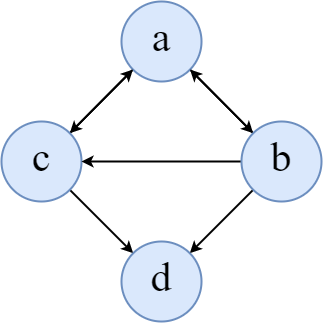
\includegraphics[width=5cm]{images/SYNASC2020_4node_7edge}
		\caption{Egy kommunikációs gráf 4 csúccsal, 3 egyszerű körrel és 1 bonyolulttal}
		\label{abra-synasc2020-4node7edge}
	\end{figure}

	Most az egyszerűség kedvéért elhagyjuk a nem egyszerű kört, és így megkapjuk az Fig.~1.-nek megfelelő \ref{abra-synasc2020-4node7edge} ábrán látható kommunikációs gráfot 3 körrel, mely a következő:
	\[ (a,b),(a,b,c),(a,c). \]
	
	Így ennek a gyenge modellje (miután minden egyes klóznak a magába foglalt teljes klózok indexeit kilistáztam \az{\eqref{eq-teljes-klozok}} képletből):
	\begin{equation*}
		\begin{split}
			WM=\{\{\neg a,b,c\} :6,7,\{\neg b,a,c,d\} :11, \\
			\{\neg c,a,d\} :9,14,\{\neg a,\neg b,c,d\} :3, \\
			\{\neg a,\neg b,\neg c,d\} :1,\{\neg a,\neg b,c,d\} :5\}. \\
		\end{split}
	\end{equation*}

	Például a $ \{\neg a,b,c\} :6,7 $ klózt úgy kaptuk, hogy a 6-os és 7-es klózokat konjugáltuk:
	$ (\neg a,b,c,\neg d)\wedge(\neg a,b,c,d)\equiv(\neg a,b,c) $
		
	%	Ezen Az eredeti gyenge modellt viszont a csomópontok teljes hosszú klózaiból kell összeállítanunk.
	A gyenge modellt a gráf teljes hosszú klózaiból kell összeállítanunk. A fent leírt szakirodalmi fogalmak alapján, onnan közelítettem meg a gyenge modell elkészítését, hogy az erős komponenseket egyetlen csomóponttal helyettesítettem. Ez pedig egy új modellt eredményezett, amit a következő fejezetben fejtek ki.
	
	\section{Kiterjesztett erős modell}\label{sec-esm}

	Ezt úgy értem el, hogy ha egy irányított gráf több \textsc{SCC}-ből áll, akkor a neki megfelelő modell mindig kielégíthető, akkor is, ha hozzáadjuk a fekete és a fehér klózokat. Ez a megállapítás független attól, hogy a gráf, melyik modelljét generáljuk le. Akkor is igaz, ha az erős, vagy ha a gyenge modell segítségével generáljuk le a neki megfelelő \textsc{SAT} példányt.
	
	Ennek az az oka, hogy az elmélet szerint akkor és csak akkor keletkezik irányított gráfból UNSAT példány, ha az irányított gráf egy \textsc{SCC}-ből áll, azaz erősen összefüggő, és hozzáadjuk a modelljéhez a fekete és a fehér klózokat.
	
	Több esetet is vizsgáltam, amikor azt irányított gráf két \textsc{SCC}-ből áll. Ezeknek az erős modelljét elkészítettem kézzel, illetve programmal is, valamint a WolframAlpha weboldalát használtam fel ezek vizsgálatára.
	
	A WolframAlpha-t már kifejtettem a \ref{kif-wolframalpha-hasznalata}.~fejezetben, így erre itt nem térnék ki minden részletére a használatával kapcsolatban.
	 
	A legegyszerűbb gráf, aminek az erős modelljét vizsgáltam, két \textsc{SCC}-ből áll. Az első \textsc{SCC} az A és a B változókból áll (számokkal kifejezve: 1, 2), a második \textsc{SCC} a C, valamint a D változókból (számokkal kifejezve: 3, 4), oly módon, hogy az első \textsc{SCC}-ből megy él a másodikba. Visszafelé természetesen nem megy él, hiszen akkor az egész gráfunkból egy nagy \textsc{SCC} lenne, amiről tudjuk, hogy egy fekete-fehér \textsc{SAT} probléma. Kutatásom során, azt találtam, hogy függetlenül attól, hogy az A-ból megy él C-be, azaz $ A \rightarrow C $, vagy A-ból megy él D-be: $A \rightarrow D$, vagy B-ből megy él C-be: $B\rightarrow C$, vagy B-ből megy él D-be: $B\rightarrow D$, mind a négy esetben az erős reprezentációnak megfelelő \textsc{DNF} formula következett:
	
	\[ (A\wedge B\wedge C\wedge D)\vee (\neg A\wedge\neg B\wedge C\wedge D)\vee (\neg A\wedge\neg B\wedge\neg C\wedge\neg D) \]
	Azaz: (A és B és C és D), vagy ($ \neg A $ és $ \neg B $ és $ \neg C $ és $ \neg D $) vagy ($ \neg A $ és $ \neg B $ és C és D)
	
	Ezt kaptam mind a négy esetben. Mint látható az első megoldás a fekete klóz negáltja, a második a fehér klóz negáltja, amiket majd kizárunk a végső megoldások közül a fekete és fehér klózok hozzá adásával, ahogy azt előírja az eredeti algoritmus Kusper Gábor és társainak cikkében\cite{am}.
	
	Ugyanakkor a harmadik megoldás nem tűnik el, és ez megfelel az eredeti elméletnek, habár az eredeti elmélet nem magyarázza meg a harmadik megoldás alakját. Ha jól megnézzük, akkor ez a harmadik megoldás: ($ \neg A $ és $ \neg B $ és C és D), azaz az első \textsc{SCC} változói negatívan szerepelnek benne, a második \textsc{SCC} változói pedig pozitívan. Megvizsgáltam több esetet is, az erős modellt legeneráltam programmal, illetve kézzel is, és a fent leírtak mindig tökéletesen beigazolódtak.
	
	Program eredménye:
	
	\begin{tabular}{cccccc}
		p & cnf & 5 & 10 & &   \\
		-1&  2 &  0&   &   &   \\
		-1&  3 &  0&   &   &   \\
		-2&  1 &  0&   &   &   \\
		-3&  4 &  0&   &   &   \\
		-4&  5 &  0&   &   &   \\
		-5&  3 &  0&   &   &   \\
		-1& -2 & -3& -4& -5& 0 \\
		 1&  2 &  3&  4&  5& 0 \\
		-1& -2 & -3& -4& -5& 0 \\
		 1&  2 &  3&  4&  5& 0 \\
	\end{tabular}

	A program írása közben, azonban sokszor futottam bele olyan hibába, hogy egy modell nem úgy néz ki, mint ahogy annak kellene a megadott paraméterek szerint. Ez látható a fentebbi táblázatban is, ahol a  legenerált \textsc{CNF} fájl a fekete és a fehér klózokat kétszer is tartalmazza, ennek oka:
	
	\begin{lstlisting}
def strong_model_literal_gen(G):
	clause = []
	bw_clause = []
	for i, j in G.edges():
		clause.append(-i)
		clause.append(j)
		clause.append(0.1)
	for i in G.nodes():
		bw_clause.append(i)
	for i in bw_clause:
		clause.append(-i)
	clause.append(0.1)
	for i in bw_clause:
	 	clause.append(i)
	clause.append(0.1)
	return clause
	\end{lstlisting}
	
	Ezt természetesen kijavítottam, és így a program már a helyes fájlt írja ki. Ez a megoldás csak egy programozói döntés kérdése, mégpedig, hogy milyen klózhalmazt akarok előállítani. A fenti esetben azt láthatjuk, hogy a program az összegyűjtött klózok halmazát (beleértve a fekete-fehér klózokat), és a fájlba író függvény által írt fekete-fehér klózokat is tartalmazza. Ez ugyan megfelelő válasz lenne az elmélethez, hogy a klózok halmaza tartalmazza a fekete-fehér klózokat is, ugyanakkor ebben az esetben redundanciát is okoz. Az alábbi programrészletben ennek a kijavítása látható:
	\newpage
	\begin{lstlisting}
def strong_model_literal_gen(G):
	clause = []
	for i, j in G.edges():
		clause.append(-i)
		clause.append(j)
		clause.append(0.1)
	return clause	
	\end{lstlisting}

A program további részében egy másik függvényben megjelennek a fájlba íráskor a fekete és a fehér klózok:
	\begin{lstlisting}
	for n in range(1, N+1):
		file_wm.write('%s ' % -n)
	file_wm.write('%s\n' % 0)
	for n in range(1, N+1):
		file_wm.write('%s ' % n)
	file_wm.write('%s\n' % 0)
	file_wm.close()
	\end{lstlisting}	
	
	A javított programmal a \textsc{CNF} fájlba írt jó eredmény:

	\begin{tabular}{cccccc}
		p & cnf & 5 & 10 & &   \\
		-1&  2 &  0&   &   &   \\
		-1&  3 &  0&   &   &   \\
		-2&  1 &  0&   &   &   \\
		-3&  4 &  0&   &   &   \\
		-4&  5 &  0&   &   &   \\
		-5&  3 &  0&   &   &   \\
		-1& -2 & -3& -4& -5& 0 \\
		1&  2 &  3&  4&  5& 0 \\
	\end{tabular}

	A következő megoldás pedig egy WolframAlpha-val készült példa, amihez ezek a bemeneti adatok:
	\[ ((A\implies B)\wedge(B\implies A)\wedge(C\implies D)\wedge(D\implies E)\wedge(E\implies C)\wedge(A\implies C)) \]
	\textsc{DNF}:
	\[ (A\wedge B\wedge C\wedge D\wedge E)\vee (\neg A\wedge\neg B\wedge C\wedge D\wedge E)\vee (\neg A\wedge\neg B\wedge\neg C\wedge\neg D\wedge\neg E) \]
	
	Mivel a megfigyelésem többször is beigazolódott, ezért a következő sejtést fogalmaztam meg:
	
	Feltételezem, hogy ha minden irányított gráf, nevezetesen G, két \textsc{SCC}-ből áll, $ S_1 $-ből, és $ S_2 $-ből, akkor ha $ S_1 $-ből legalább egy él vezet $ S_2 $-be, akkor függetlenül az élek számától, illetve, hogy konkrétan az élek melyik $ S_1 $-ben lévő csomópontból, melyik $ S_2 $-ben lévő csomópontba vezetnek, akkor G-nek a \textsc{SAT} modelljének pontosan ez az egy megoldása lesz, amennyiben a modellhez hozzáadjuk a fekete és a fehér klózokat is: $ \neg S_1\wedge S_2 $, ahol $ \neg S_1 $ ez a formula: $\neg A_1 \wedge \neg A_2\wedge\dots\wedge\neg A_k$, ahol $ S_1 $ csomópontjai: $ A_1,A_2,\dots,A_k $, és $ S_2 $ ez a formula: $ B_1\wedge B_2\wedge\dots\wedge B_m $, ahol $ S_2 $ csomópontjai: $ B_1,B_2,\dots,B_m $.
	
	Sajnos a sejtésemet egyelőre nem sikerült bizonyítani, de az általam kipróbált minden példára működött, akkor is, ha az erős modellt generáltam, akkor is ha a gyengét, akkor is, ha bármely másikat, azaz szerintem ez egy fontos felismerés.
	
		\subsection{A kutatás eredménye, általánosítás}

	A fenti megfigyelésből az az ötletem támadt, hogy az összes \textsc{SCC}-t egy-egy csomóponttal helyettesítem, azért hogy kisebb bonyolultságú gráfokat kelljen kezelnem, amelyre az általam megírt kódok is rövidebb idő alatt futnak le.

	Az első út, amit kipróbáltam, annak a vizsgálata, hogy hogyan lehet kiegészíteni a legenerált \textsc{SAT} modelleket, oly módon, hogy a fent ismertetett tulajdonság megmaradjon, azaz $\neg S_1$ és $ S_2 $ megoldás maradjon, de az egyes \textsc{SCC}-ket már egy változó képviselje (azaz a \textsc{DIMACS} fájlokban egy szám).
	%todo képek milyen szélesek legyenek?
	\begin{figure}[!ht]
		\centering
		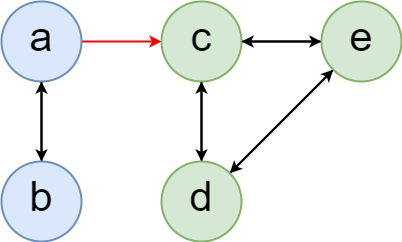
\includegraphics[width=5cm]{images/sajat_pelda_5node_9edge}
		\caption{Eredeti gráf, benne az összes \textsc{SCC}.}
		\label{abra-sajatpelda-eredeti-5-9graf}
	\end{figure}

	\begin{table}[h!]
		\centering
		\begin{tabular}{cccccccc}
		p & cnf & 7 & 5 & & & &  \\
		-1&-2& 6& 0&  &  &  &  \\
		-3&-4&-5& 7& 0&  &  &  \\
		-6& 7& 0&  &  &  &  &  \\
		-1&-2&-3&-4&-5&-6&-7& 0 \\
		1& 2& 3& 4& 5& 6& 7& 0 \\
		\end{tabular}
		\caption{\label{table-esm-cnf}A \textsc{DIMACS} formátumú .cnf fájl}
	\end{table}
	
	Hosszas próbálkozás után a következő ötletem támadt. Rávilágítottam, hogy erős komponensenként egy csomóponttal is leírhatjuk:
	
	\begin{figure}[!ht]
		\centering
		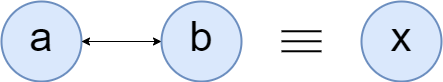
\includegraphics[width=5cm]{images/sajat_pelda}
		\caption{$ a\leftrightarrow b\equiv x$, azaz egy \textsc{SCC}-t helyettesíthetek egyetlen változóval.}
		\label{abra-sajatpelda-ab-x}
	\end{figure}
	
	Ha az ehhez tartozó következő bemeneti adatokat adjuk meg a WolframAlpa-nak:
	\[ (A\implies B)\wedge(B\implies A)\wedge(A\vee B \implies X)\wedge(\neg A\vee\neg B\implies\neg X) \]

	Akkor annak a \textsc{DNF}-ben a leegyszerűsített változata:
	\[ (A\wedge B\wedge X)\vee(\neg A\wedge\neg B\wedge\neg X) \]	
	Azaz: ((A=>B) és (B=>A) és (A vagy B => X) és ($ \neg A $ vagy $ \neg B $ => $ \neg X $)), ahol az A, és B változókból áll az \textsc{SCC}, valamint X változóval lehet helyettesíteni az \textsc{SCC}-t.
	
	A fenti kiegészítést úgy lehet megkapni, hogy az \textsc{SCC} fehér klóza implikálja az $ X $ literált, a fekete klóza pedig a $ \neg X $ literált. Ezzel a kiegészítéssel az \textsc{SCC}-nek ugyanúgy csak két megoldása van, mint a kiegészítés előtt. A két megoldás, a fekete és a fehér hozzárendelése, annyi kiegészítéssel, hogy most már szerepel bennük az X atom is. Azaz a két megoldás: $ (A \wedge B \wedge X) $, valamint $ (\neg A \wedge \neg B \wedge \neg X) $
	
	Ezzel a kiegészítéssel azt lehet nyerni. hogy ha van két \textsc{SCC}, mondjuk $ S_1 $ és $ S_2 $, ekkor $ S_1 $-et az $ X $-el egészítem ki és $ S_2 $-t az $ Y $-al, akkor minden élt, ami $ S_1 $-ből $ S_2 $-be megy, azt le tudom írni egy darab klózzal: $ (X\implies Y) $, azaz $ (\neg X\vee Y) $, ami kisebb \textsc{SAT} modellhez vezethet.
	
	\begin{figure}[!ht]
		\centering
		
\includegraphics[width=3cm]{images/sajat_pelda_5_9_to_esm}
		\caption{Leegyszerűsített gráf, behelyettesítés után. Kibővített erős modell (\textsc{ESM})}
		\label{abra-sajatpelda-59to-esm}
	\end{figure}

	Ráadásul a modelleknek az általam vizsgált összes tulajdonsága megmarad.
	
	Egy ettől is egyszerűbb megoldás, ha az első \textsc{SCC}-t az 1-es számmal, $ A $ változóval, a másodikat pedig a 2-es számmal, B változóval helyettesítem. Így rendre egy-egy változót (de mindegyikhez különbözőt) rendelek az erős komponensekhez. Ebből generálok egy erős modellt, majd ennek az erős modellnek a megoldásaimban visszahelyettesítem az \textsc{SCC}-k eredeti változóit a megoldásban kapott előjellel. Így akár nagyon nagy, több ezres irányított gráfok megoldása is milliszekundumok alatt lehetséges.
	\newpage
	
	Ehhez természetesen meg kell találni az összes \textsc{SCC}-t és a köztük lévő kapcsolatokat, ami nem egyszerű feladat. Változatos a gráfok minden formája. Egy általánosított modellt próbáltam meghatározni \ref{abra-sajatpelda-altalanos}.~ábrán, ami az összes lehetséges alakot lefedi.
	
	\begin{figure}[!ht]
		\centering
		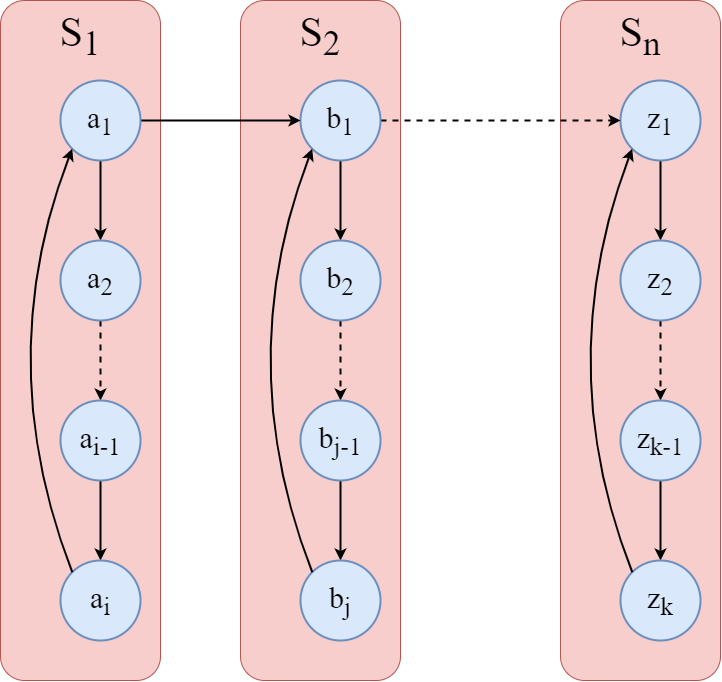
\includegraphics[width=10cm]{images/sajat_pelda-altalanos}
		\caption{Egy gráf leírása, akár mennyi \textsc{SCC} esetén.}
		\label{abra-sajatpelda-altalanos}
	\end{figure}	

	Ehhez az ihletet Johnson cikkéből \cite{johnson} merítettem. Itt említi meg, hogy Tarján algoritmusára \cite{tarjan} mik a legrosszabb eshetőségek, ehhez volt pár ábra, amit az általánosításkor jó alapnak bizonyult.

	\begin{figure}[!ht]
		\centering
		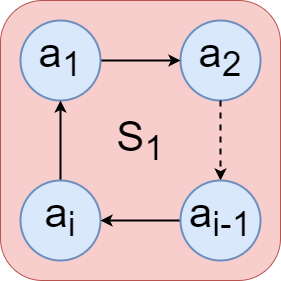
\includegraphics[width=5cm]{images/sajat_pelda-altalanos_scck_a}
		\caption{Egy lehetséges erős komponens alakja (a) változóval jelölve, az $ S_1 $-es erős komponensben.}
		\label{abra-sajatpelda-altalanos_scck_a-verzio}
	\end{figure}
	\newpage	
	Az \textsc{SCC}-k megtalálására természetesen több módszer is létezik. Én kicsit más úton indultam el, mint amit a konzulensem kért tőlem. Szerintem ez is a probléma megoldásának egyik lehetséges verziója, hiszen új megvilágításban, és más megközelítéssel vittem az ő munkájukat tovább. Ezekről kóddal együtt a következő fejezetben részletesebben fejtem ki mondanivalómat.
	\begin{figure}[!ht]
		\centering
		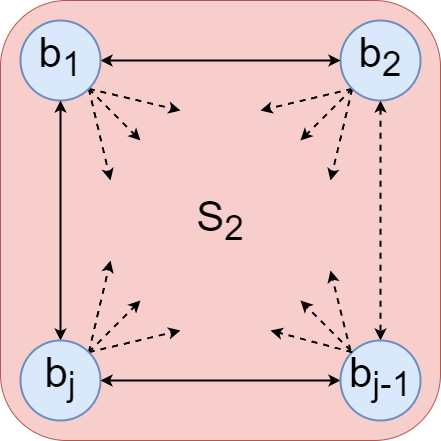
\includegraphics[width=8cm]{images/sajat_pelda-altalanos_scck_b2}
		\caption{Egy lehetséges erős komponens alakja (b) változóval jelölve, az $ S_2 $-es erős komponensben.}
		\label{abra-sajatpelda-altalanos_scck_b-verzio}
	\end{figure}
	
\chapter{Szoftver}
	\section{Kiindulási pont}
	Ebben a fejezetben a programból kiemelt sorok szerepelnek, úgyhogy nem minden részlet van kifejtve és leírva.
	
	A programozási feladat, ami egy saját készítésű \textsc{SAT} megoldó a CSFLOCK, egy Java-ban írt program. A bemeneti formátuma, amivel dolgozik az egy .cnf fájl, aminek több fajtája is ismert. Munkám során ilyen fájlokat tudok generálni a graph\_cnf\_GEN nevű programok segítségével. Ezek különböző verziókban készültek el, ahogyan előrehaladtunk. Az alapokat korábban Biró Csaba egyetemi docens készítette el konzulensemmel közös munkájuk során.
	
	Ez a graph\_cnf\_GEN\_0.8.py \cite{github-py08} fájl névre hallgat. Ebből az alapból kiindulva tanulmányoztam a fájl szerkezetét. Tartalmilag néhány része nem volt teljesen kifejtve, ez a későbbi verzióban már letisztult és használható formában jelenik meg. Az eredeti fájlnak nem az összes funkcióját ültettem át, hiszen a hangsúlyt a kutató munkára helyeztem.
	
	A program egy részének lefordítása futási problémákba ütközött, nem produkálta a teljes működést. Ennek a kijavítása ugyan fontos lépés a modellek pontos működéséhez. A kód megfelelő beállítása és finomhangolása rendkívül összetett folyamat, mivel \az{\cite{github-py08}} egy korábbi, 2.0 Python-ban készülhetett, ezért kompatibilitás hiánya miatt hibára futott az újabb Python 3.0 feletti verzióban.
	
	\begin{lstlisting}
for i in xrange(len(clauseSet)):
	if i <> 0:
	\end{lstlisting}

	Néhány kódrészlet pedig azért futott hibára, mert eredetileg még nem volt, vagy nem pontosan volt definiálva néhány változó:
	
	\begin{lstlisting}
isStrConn
graph_dens
g = networkx.DiGraph()
cic = find_cycle(g)
for i in range(0,len(cic)):
	a_cycle.append(cic[i][0])
	\end{lstlisting}

	A program megértése során számomra az utolsó sor volt a legnehezebb, mivel bonyolultsága miatt pontos jelentését, és feladatát a rendelkezésre álló időben nem tudtam megfejteni. Felkeltette érdeklődésemet, és ha lehetőségem adódik rá, folytatni fogom vizsgálatát, mivel szerintem ez a kulcs a további modellek generálásához. A programban, ugyanebben a mélységű behúzásban, de kicsit később ezeket a sorokat láthatjuk:
	
	\begin{lstlisting}
if find_cycle(g):
	isCici=len(find_cycle(g))
	\end{lstlisting}

	A program ezen sorainak vizsgálata alatt azt feltételeztem, hogy nem megoldható feladat az előző, és a felette lévő kódrészletekben a find\_cycle() függvény futtatása során háromféle érték visszaadása. A cic változó értéke a megtalált körök, valamint egy Boolean érték (kör találása esetén), majd egy harmadik esetben annak a körnek a hosszát megadni, vagy hogy mennyi kör van a ,,g'' irányított gráfban. Ezeket a kódrészleteket kezdetben még nem tudtam átfordítani, emiatt úgy döntöttem, hogy külön fájlban, új verzió számmal elkezdem a nulláról felépíteni a projektet. A teljes kód átdolgozásáig hosszú út vezet, viszont a következő részben arról írok, amit a kód átfordítása során megértettem és kiviteleztem, hogy futtatás során a program érthetően és hiba nélkül működjön.
	
	\section{A kiterjesztett erős modell Python megoldásai}
	
	Nagyon sok verzión ment át a kód, mielőtt idáig eljutott, de végül úgy működik, ahogyan azt elgondoltam és most láthatjuk. Ezért kapott új verzió számot is az átdolgozott rész. Használtam előre megírt könyvtárakat is, amik nagyban segítették a munkámat.

	\begin{lstlisting}
from itertools import tee, islice, chain
import networkx as nx
import pylab
	\end{lstlisting}

	Sorban, ahogyan felhasználtam őket: indexeléshez és pontosabb lista bejáráshoz használom az első sor könyvtárait. A \texttt{NetworkX} könyvtár a legfontosabb munkám során, hiszen minden ami a gráfokhoz kapcsolódik, azt ebből merítettem. Használata közben a fejlesztők felé jeleztem saját github repository-jukba írt issue-val \cite{link-github-issue}, hogy néhány példával egészítsék ki a condensation függvényük leírását, ami nagyban megkönnyítheti a kód pontos használatának a megértését. Ez a könyvtár segít gráfot építeni, módosítani, keresni benne, csomópontokat rendezni és még sok más hasznos osztályt és függvényt is tartalmaz, de ezekről majd később beszélek részletesen. Nem szabad megfeledkeznünk az utolsó sorról sem, ami a gráfok fájlba írását segíti. Rengeteg matematikai műveletet tartalmaz és segít kezelni, formázni a gráfunkat, hogy képeket, és .cnf fájlokat készíthessünk belőle.
	
	A következő részletben a fő elemet láthatjuk. Ebben indítom, el az összes folyamatot és módosítom a bemeneti gráfot.
	
	\begin{lstlisting}
def main():
	edges = []
	
	edges.append((2,1))
	edges.append((1,3))
	edges.append((1,4))
	edges.append((3,2))
	edges.append((4,5))
	edges.append((5,4))
	
	g = nx.DiGraph(edges)
	Literals = expanded_strong_model_literal_gen(g)
	model_to_cnf_file(g, Literals, "ESM")
	Literals = strong_model_literal_gen(g)
	model_to_cnf_file(g, Literals, "SM")
	
main()
	\end{lstlisting}

	
	Kell egy üres lista, amihez különleges módon adom hozzá az éleket. Az éleknek megfelelő számokat a \texttt{NetworkX} fejlesztői egy konvenció alapján adják át \cite{link-github-issue}, legalábbis ebből a korábban említett issue-ból ezt sejtem. Ebben a következő használatot javasolják:
	
	\begin{lstlisting}
edges = []
edges.append(((2,1),(1,3),(1,4),(3,2),(4,5),(5,4)))
	\end{lstlisting}
	
	Én azért használom hosszabban leírva, mert számomra sokkal átláthatóbb, jobban szerkeszthető és követhető, hogy miből áll a gráfunk. Egy szám egy csomópontnak felel meg. Egy számpáros pedig azt mutatja, hogy a két csomópont közt él van. Ezek listáját átadom a \texttt{NetworkX} irányított gráf generáló algoritmusnak, az elkészült gráfot pedig eltárolom egy változóban. Ezek után saját függvényeimet hívom meg, és elkészítem a modellnek megfelelő literálok halmazát. Végül az elkészült literálokat adom át a Biró Csaba tanár úr által korábban elkészített .cnf fájlt generáló függvénynek.
	\newpage
	Az általam készített függvény a következő:

	%próbát megér caption csomag + label
	%Az általam megírt ESM modell generáló
	\begin{lstlisting}
def expanded_strong_model_literal_gen(G):
	dagg = nx.condensation(G)
	mem = nx.get_node_attributes(dagg, "members")
	print("members: ", mem)
	clause = []
	edges = list(dagg.edges())
	if len(edges) == 0:
		for i in mem.values():
			while i:
				clause.append(-i.pop())
		clause.append(0.1)
		print("Careful! All are negative literals.")
		return(clause)
	else:
	\end{lstlisting}\label{kod-nx-condensation}

	A \texttt{print} függvényt használom állandó visszajelzésnek, mivel sokszor modellgenerálást váltok, ezért jó látni, melyikkel dolgozom jelenleg, és milyen rész információk kapcsolódnak ehhez. A megfelelő bemenetet használtam-e, azaz csak az éleket kell átadni, és azt is figyelni kell, hogy egy csomópont nem mutathat magára. Ezek után a \texttt{NetworkX} könyvtárában a \texttt{condensation} függvényt használva visszakapom a gráfom kondenzációját, amit egy változóban eltárolok. Ezen belül létrejött egy szótár, amiben tárolja az erős komponensekhez hozzárendelt új csomópontokat, és ezeknek az eredeti csomópontjait. A erősen összetett komponenseket Tarján Róbert algoritmusával \cite{tarjan} és Nuutila módosításával \cite{nuutila} találja meg. Ezekkel az adatokkal már egyszerűbb dolgunk van. Ha az egész szótárt bejárjuk, akkor láthatjuk, hogy hány új él van. Ha nincs benne él, akkor az egész gráf egy erősen összetett komponens volt, és minden csomópontot negatívként adunk hozzá a klózhalmazhoz.

	Ennek ,,else'' ágában:
	\begin{lstlisting}
for prev, curr in previous(mem.items()):
	if len(curr[1]) > 1:
		for pre, cu in previous(curr[1]):
			if pre == None:
				firs = cu
				continue
			if (pre, cu) in G.edges():
				clause.append(-pre)
				clause.append(cu)
				clause.append(0.1)
			if (cu, pre) in G.edges():
				clause.append(-cu)
				clause.append(pre)
				clause.append(0.1)
			if (cu, firs) in G.edges() and pre != firs:
				clause.append(-cu)
				clause.append(firs)
				clause.append(0.1)
			if (firs, cu) in G.edges() and pre != firs:
				clause.append(-firs)
				clause.append(cu)
				clause.append(0.1)
	if prev == None:
		continue
	if (prev[0], curr[0]) in edges:
		print("edge goes from previous to current")
		for i in prev[1]:
			clause.append(-i)
		for i in curr[1]:
			clause.append(i)
		clause.append(0.1)
	
	if (curr[0], prev[0]) in edges:
		print("edge goes from current to previous")
		for i in curr[1]:
			clause.append(-i)
		for i in prev[1]:
			clause.append(i)
		clause.append(0.1)
	\end{lstlisting}	
	
	Az általam írt függvény fő része végigmegy a szótár előző és jelenlegi elemein. Az első elem előtt nincs semmi, ezért a \texttt{prev} értéke kezdetben \texttt{None}. Ebben az iterációban a legelső erős komponens elemein végigmegyek, ha egynél több eleme van, akkor hozzáadom annak literáljait a klózhalmazhoz. Csak ezek után lépek a következő iterációra, ahol ugyanezeket a lépéseket megismételem, annyi különbséggel, hogy most már az erős komponensek közti éleket is beleírom a klózhalmazba. A klózhalmaz tulajdonképpen egy lista, amiben a halmaz elemeit egy különleges értékkel határolom el.
	
	Ezek után a fájlba a határoló karakter segítésével, egy másik metódussal, a megfelelő \textsc{DIMACS} formátumban írom ki a lista elemeit.

	\begin{table}[h!]
		\centering
		\begin{tabular}{ccccc}
		p & cnf & 4 & 8 &   \\
		-1 &  2 &  0 & &\\
		-2 &  1 &  0 & &\\
		-1 &  3 &  0 & &\\
		-3 &  1 &  0 & &\\
		-2 &  3 &  0 & &\\
		-1 & -2 & -3 &  4 & 0\\
		-1 & -2 & -3 & -4 & 0\\
		 1 &  2 &  3 &  4 & 0\\
		\end{tabular}
		\caption{A \textsc{DIMACS} formátumú .cnf fájl első verziója}
	\end{table}
	
	%\subsection{A legelső megvalósítás}
	% 3.2 tartalma
	%\subsection{A második megvalósítás}
	% ami itt jün
	\subsection{Az első verzió egy továbbfejlesztett megoldása}
	
	Ahogyan azt korábban bemutattam a helyes eredmény \az{\ref{table-esm-cnf}}.~táblázatban látható. Ez alapján azt vettem észre, hogy szükséges módsoításokat végezzek. Előszőször is hatékonyabbá és érthetőbbé tettem azt az esetet, amikor csak egy elemből áll a leegyszerűsített gráf.
	\begin{lstlisting}
clause = []
if len(dagG.edges()) == 0:
	for cycle in mem.items[1]:
		clause.append(-cycle)
	#clause.append(mem.items[0])
	clause.append(0.1)
	return clause
	\end{lstlisting}
	
	Itt fontos, hogy egy változót kihagytam és csak egy ciklusmag van, amivel erőforrást spóroltam. A kikommentelt részletet még miközben írtam átgondoltam, hogy ha csak egy SCC van, akkor nem kell hozzáadni a klózhoz azt, amivel az egészet helyettesíteném. Még további teszteket igényel, hogy kipuhatoljuk milyen eredményekkel jár, ha ez az eset fut le. Legvalósínűbb megoldásnak a NetworkX megoldását találom, miszerint a 0 hosszú/nagyságú/méretű/élű,egyszerűsített gráf esetén, csak lépjen ki a metódusból.
	
	A \ref{kod-nx-condensation}.kódrészletben a 2. sorában egy apró ám hasznos változást vezettem be. Az említett NetworkX-es condensation függvényt kiegészítettem egy 3. opcionális paraméterrel, ami egyszerűen a számozás kezdetét határozza meg. Azaz honnan indítsa az új SCC-ket helyettesítő csomópontok számozását. Egy kis kutatás és utánanézés kellett hozzá, hogy az eredeti függvényt ki tudjam egészíteni a megfelelő módon. A válasz megepően rövid volt a korábbi elképzeléseimhez képest:

\begin{lstlisting}
	#dagG = condensation(G)
	dagG = condensation(G, None, G.number_of_nodes() + 1)
\end{lstlisting}

	Alapértelmezésben, ahogy eddig is 0-tól indul a számozás, ha nem adunk át értéket. Ez az extra paraméter ahhoz kell, hogy a condensation függvényben amikor az SCC-ket számoljuk, akkor az enumerate függvény honnan kezdje a számozást.

\begin{lstlisting}
def condensation(G, scc=None, offset=0):
	"""Description"""
	if scc is None:
		scc = nx.strongly_connected_components(G)
	mapping = {}
	members = {}
	C = nx.DiGraph()
	# Add mapping dict as graph attribute
	C.graph["mapping"] = mapping
	if len(G) == 0:
		return C
	for i, component in enumerate(scc, offset):
		members[i] = component
		mapping.update((n, i) for n in component)
	number_of_components = i + 1
	C.add_nodes_from(range(number_of_components))
	C.add_edges_from(
		(mapping[u], mapping[v]) for u, v in G.edges() if mapping[u] != mapping[v]
	)
	# Add a list of members (ie original nodes) to each node (ie scc) in C.
	nx.set_node_attributes(C, members, "members")
	return C	
\end{lstlisting}
	Így elég volt csak az offset változót a jó helyre hozzátennem.Habár ez elég egyszerűnek tűnik, ennek megértése és átlátása alapos értelmezést és odafigyelést igényel. Ebből a NetworkX csapatának egy külön issue-t/pull-request-et is küldtem. %\cite[]{link-github-contribution}
	%todo Csináld meg a hivatkozást. Nézzem át/írjam le résletesebben a kódot

	\section{Célok a jövőben, variációk a fejlesztésre}
	
	Még rengeteg metódus és függvény van, amit meg lehet írni az eredeti kód \cite{github-py08} alapján. Jómagam is terveztem folytatni a modellek átírását az új Python verzióra, valamint implementálni az értelmezését. A jelenlegi kódot is célszerű karbantartani, kitakarítani, egyszerűsíteni. Sok lehetőség van még benne. Úgy érzem, hogy a jelenleg elkészült programkód értelmezése egyszerű, könnyen bővíthető és használatához nem kell külön az én segítségemet kérni.
	
	A kód legvége mintegy ötletbörzeként, tartalmaz egy pár tesztesetet, ezek kiinduló pontjai lehetnek egy újabb fejlesztésnek is. Külön fájlba gyűjtve, sok elemet tartalmazó, sokoldalú teszteset gyűjtemény hozható létre belőle. A teszteseteket, ahogy tőlem is kérték meg lehetne írni a \texttt{NetworkX} csapatának annotálásával, stílusával és konvenciójával. A további gráfok generálására érdemes kibővíteni a teszteseteket, hogy lefedjék az összes eshetőséget és általánosságban beszélhessünk a gráfokról. Erre azért van szükség, hogy biztosan meg tudjuk állapítani, hogy jó .cnf fájlt ad a tanáraim által korábban létrehozott véletlenszerű, irányított gráf generátor, ami \textsc{WSN} hálózatokat \cite{am} ír le az által, hogy kommunikációs gráfokat generál.
	
	További fejlesztés lehetőségeként a változók értékeinek nyomon követésére a programba beépített modult lehetne használni a \texttt{print} függvények helyett.
	
	Az eredeti programkódból szakdolgozatom felhasználásával tovább lehet fejleszteni a gyenge modellt akár kiemeléssel, kiegészítéssel, átalakítással, mivel a jelenlegi kód megírásakor végül nem ezt a részt dolgoztam ki. Szívesen folytatom a munkát a későbbiekben a többi modell és az algoritmus Python nyelvre való átfordításával, amennyiben ez támogatja a fejlesztők munkáját. Fejlesztését lehet folytatni a többi modellnek is.

	A \textsc{SAT} megoldóhoz is, amit a konzulensem Java programozási környezetben írt meg és \textsc{CSFLOC} névre hallgat számtalan fejlesztési lehetőség társul. Úgy tudom abban is lehet fejlesztéseket eszközölni, lásd gyorsabb körkereső algoritmus implementálása \cite[Johnson]{johnson} algoritmusa alapján. A gyenge modellhez pedig minden lehetőség adott, és már csak egy karnyújtásnyira van, hogy annak is láthassuk a végeredményét.	A \textsc{CSFLOCK} teszteléséhez az alappillérek, azok a modellek, melyek még fejlesztésre várnak és amelyek szükségesek ahhoz, hogy ez a projekt tovább fejlődjön.
	
\chapter*{Összegzés}\addcontentsline{toc}{chapter}{Összegzés}
	Szakirodalmat fordítottam, értelmeztem és dolgoztam fel.
	Ezekből kiindulva, néhány alap fogalmat leírtam és magyarázó szöveggel láttam el.


	Egy régebbi, elmaradt kódot élesztettem, értelmeztem újra.
	Ezzel párhuzamosan elsajátítottam a Python programozási nyelv alapjait, melynek segítségével közelebb kerültem az eredményeim eléréséhez.
	Sok munka árán eljutottam egy modell generálásáig, amire azt hittem a gyenge modell, ám kiderült, hogy az erős modellt általánosítottam.
	Ehhez a szabályokat, a modell összetételét és a formális megfogalmazását is elkészítettem.
	Általam készített képekkel, ábrákkal próbáltam érthetőbbé, színesebbé tenni a szakirodalmat.
	Ezekkel igyekeztem elmagyarázni a modellt és annak működését.
	A kód, amit fejlesztettem jó fájlokat generál. Több, használható tesztesetem is van.
	
	Folytatásként külön részleteztem néhány sorát az általam írt kódoknak, a jobb érthetőség érdekében, valamint ez a kód dokumentációja is.

	Az általam használt linkek külső forrásból vannak, nem én tartom fent az url-ek mögötti weboldalakat, ezért a linkek idővel elavulhatnak.
	
\chapter*{Köszönetnyilvánítás}

	Nagy hálával és köszönettel tartozom konzulensemnek Dr.~Kusper Gábornak és tanáromnak Biró Csabának, amiért megadták az alapokat szakdolgozatom megírásához, segítették egyetemi tanulmányaimat, és támogatták előre haladásomat.

	Köszönöm minden egyetemi tanáromnak az építő kritikát, a türelmet és az odaadást, amivel tanítottak.
	
	Köszönöm szüleimnek, hogy mindig mellettem álltak. Köszönöm lelki és anyagi támogatásukat, a néha kemény szavakat, amivel kitartásra ösztönöztek. Nem utolsó sorban türelmüket, hiszen az ő segítségük nélkül nem jutottam volna el idáig.
	
	Köszönetet mondok a barátnőmnek és családjának, a barátaimnak, akiket jó párszor a végletekig igénybe vettem, végighallgattak, segítséget kérhettem tőlük Discordon \cite{dc}, akármilyen későn is hívtam fel őket.
	
	Hálás szívvel gondolok mindazokra, akik hozzájárultak céljaim eléréséhez.
	
\begin{thebibliography}{2}
	\addcontentsline{toc}{chapter}{\bibname}
	%cím, író\\cikk, oldalszám, év
	\bibitem{tarjan}\textsc{Depth-First Search and Linear Graph Algorithms
	\\Robert Tarjan}
	\\SIAM Journal on Computing 1972 1:2, 146-160
	\\\url{https://epubs.siam.org/doi/10.1137/0201010}

	\bibitem{johnson}\textsc{Finding All the Elementary Circuits of a Directed Graph
	\\Donald B.~Johnson}
	\\SIAM Journal on Computing 1975 4:1, 77-84
	\\\url{https://epubs.siam.org/doi/10.1137/0204007}
	
	\bibitem{nuutila}\textsc{Finding the strongly connected components in a directed graph.}
	\\\textsc{E. Nuutila and E. Soisalon-Soinen }
	\\Information Processing Letters 49(1): 9-14, (1994)
	
	\bibitem{am}\textsc{G.~Kusper, T.~Balla, C.~Biró, T.~Tajti, Z.~G.~Yang and I.~Baják, "Generating Minimal Unsatisfiable SAT Instances from Strong Digraphs,"}
	\\2020 22nd International Symposium on Symbolic and Numeric Algorithms for Scientific Computing (SYNASC), 2020, pp. 84-92, 
	\\doi: 10.1109/SYNASC51798.2020.00024.
	
	\bibitem{sat-solving-50}\textsc{G.~Kusper, C.~Biró and G.~B.~Iszály, "SAT solving by CSFLOC, the next generation of full-length clause counting algorithms,"}
	\\2018 IEEE International Conference on Future IoT Technologies (Future IoT), 2018, pp. 1-9, 
	\\doi: 10.1109/FIOT.2018.8325589.
	
	\bibitem{github}Saját GitHub oldala a szakdolgozatomnak:
	\\\url{https://github.com/Moss4t/Szakdolgozat}
	
	\bibitem{github-py08}A graph\_cnf\_GEN\_0.8.py fájl ezen a linken található:
	\\\url{https://github.com/Moss4t/Szakdolgozat/blob/main/gen%20py/graph_cnf_GEN_0.8.py}
		
	\bibitem{link-drawio}A draw.io weboldalas elérhetősége:
	\\\url{https://www.draw.io}
	
	\bibitem{link-wolframalpha}A WolframAlpha weboldalas elérhetősége:
	\\\url{https://www.wolframalpha.com}
	
	\bibitem{link-github-issue}Az általam elindított issue GitHub-on
	\\\url{https://github.com/networkx/networkx/discussions/5446}, amiből kiindult beszélgetés, és az issue:
	\\\url{https://github.com/networkx/networkx/issues/5449}		
	\bibitem{dc}Discord weboldala:
	\\\url{https://discord.com}
\end{thebibliography}
	
	% Aláírt, szkennelt nyilatkozat beillesztése a szakdolgozat végére
	
\includepdf[pagecommand={\thispagestyle{empty}}]{nyilatkozat.pdf}
\end{document}